% Practice Test 08 — Virginia Edition
% Questions: 30 (21 MC + 9 SA)
% Generated by scripts/generate_practice_tests.py

\begin{practiceQuestion}{1-4-q13}{mc}
\begin{questionText}
A factory produces $24$ toys per hour. Which equation gives the number of toys $t$ in $h$ hours?
\end{questionText}
\choiceA{$t = h + 24$}
\choiceB{$t = 24h$}
\choiceC{$h = 24t$}
\choiceD{$t = \frac{24}{h}$}
\correctAnswer{B}
\explanation{Toys $= 24 \times$ hours, so $t = 24h$.}
\end{practiceQuestion}

\begin{practiceQuestion}{2-1-q21}{sa}
\begin{questionText}
$56$ is $80\%$ of what number?
\end{questionText}
\correctAnswer{$70$}
\explanation{Divide: $56 \div 0.80 = 70$.}
\end{practiceQuestion}

\begin{practiceQuestion}{2-2-q26}{gmc}
\begin{questionText}
The table below shows the results of a class vote for a field trip. What percent of the class voted for the zoo?

\begin{center}
\begin{tabular}{|l|c|}
\hline
\textbf{Destination} & \textbf{Votes} \\
\hline
Zoo & $18$ \\
\hline
Museum & $12$ \\
\hline
Aquarium & $15$ \\
\hline
Park & $15$ \\
\hline
\end{tabular}
\end{center}
\end{questionText}
\choiceA{$18\%$}
\choiceB{$25\%$}
\choiceC{$30\%$}
\choiceD{$36\%$}
\correctAnswer{C}
\explanation{Total votes: $18 + 12 + 15 + 15 = 60$. Zoo: $\frac{18}{60} = \frac{p}{100}$ → $p = 30\%$.}
\end{practiceQuestion}

\begin{practiceQuestion}{2-3-q10}{mc}
\begin{questionText}
A car's value decreased from $\$18{,}000$ to $\$15{,}300$. What is the percent decrease?
\end{questionText}
\choiceA{$12\%$}
\choiceB{$15\%$}
\choiceC{$18\%$}
\choiceD{$20\%$}
\correctAnswer{B}
\explanation{Change: $18{,}000 - 15{,}300 = 2{,}700$. Percent decrease: $2{,}700 \div 18{,}000 = 0.15 = 15\%$.}
\end{practiceQuestion}

\begin{practiceQuestion}{2-7-q17}{mc}
\begin{questionText}
A farmer estimated his field would produce $500$ bushels of corn. The actual harvest was $600$ bushels. What is the percent error (rounded to the nearest tenth)?
\end{questionText}
\choiceA{$10\%$}
\choiceB{$16.7\%$}
\choiceC{$20\%$}
\choiceD{$25\%$}
\correctAnswer{B}
\explanation{$\frac{|500 - 600|}{600} \times 100 = \frac{100}{600} \times 100 \approx 16.7\%$.}
\end{practiceQuestion}

\begin{practiceQuestion}{3-2-q27}{gmc}
\begin{questionText}
Which number line correctly models $(-4) + (-3)$?

\begin{center}
\begin{tikzpicture}
  % Model A
  \node[left] at (-7.5,2) {\textbf{A:}};
  \draw[thick,->] (-7,2) -- (3,2);
  \foreach \x in {-6,...,2} \draw (\x,2.1) -- (\x,1.9) node[below] {\footnotesize $\x$};
  \draw[thick,->,funRed] (-4,2.4) -- (-7,2.4);

  % Model B
  \node[left] at (-7.5,0) {\textbf{B:}};
  \draw[thick,->] (-7,0) -- (3,0);
  \foreach \x in {-6,...,2} \draw (\x,0.1) -- (\x,-0.1) node[below] {\footnotesize $\x$};
  \draw[thick,->,funBlue] (-4,0.4) -- (-1,0.4);
\end{tikzpicture}
\end{center}
\end{questionText}
\choiceA{Model A}
\choiceB{Model B}
\choiceC{Both are correct}
\choiceD{Neither is correct}
\correctAnswer{A}
\explanation{$(-4) + (-3)$ means start at $-4$ and move $3$ units left (adding a negative). Model A shows the arrow going from $-4$ to $-7$, which is correct.}
\end{practiceQuestion}

\begin{practiceQuestion}{3-3-q04}{mc}
\begin{questionText}
What is $(-4) - (-4)$?
\end{questionText}
\choiceA{$-8$}
\choiceB{$8$}
\choiceC{$0$}
\choiceD{$-16$}
\correctAnswer{C}
\explanation{$(-4) - (-4) = (-4) + 4 = 0$. Any number minus itself equals $0$.}
\end{practiceQuestion}

\begin{practiceQuestion}{3-4-q12}{mc}
\begin{questionText}
What is $-1.25 - (-3.75)$?
\end{questionText}
\choiceA{$-5.00$}
\choiceB{$-2.50$}
\choiceC{$2.50$}
\choiceD{$5.00$}
\correctAnswer{C}
\explanation{$-1.25 - (-3.75) = -1.25 + 3.75 = 2.50$.}
\end{practiceQuestion}

\begin{practiceQuestion}{4-3-q25}{sa}
\begin{questionText}
Expand and simplify $-4(a - 2) + 3(a + 5) - 7$.
\end{questionText}
\correctAnswer{$-a + 16$}
\explanation{Expand: $-4a + 8 + 3a + 15 - 7$. Combine: $(-4a + 3a) + (8 + 15 - 7) = -a + 16$.}
\end{practiceQuestion}

\begin{practiceQuestion}{4-4-q03}{mc}
\begin{questionText}
Factor $15a - 10$.
\end{questionText}
\choiceA{$5(3a - 2)$}
\choiceB{$5(3a + 2)$}
\choiceC{$3(5a - 10)$}
\choiceD{$10(a - 1)$}
\correctAnswer{A}
\explanation{GCF of $15$ and $10$ is $5$. Factor: $15a \div 5 = 3a$ and $-10 \div 5 = -2$. Result: $5(3a - 2)$.}
\end{practiceQuestion}

\begin{practiceQuestion}{5-4-q30}{gsa}
\begin{questionText}
A number line shows a point at $x$. The equation $\dfrac{x}{4} + 1.5 = 5$ tells you how to find $x$. Solve and identify where $x$ is on the number line.

\begin{center}
\begin{tikzpicture}[scale=0.45]
  \draw[thick,->] (-2,0) -- (18,0);
  \foreach \x in {0,2,...,16} {
    \draw (\x,0.2) -- (\x,-0.2) node[below] {$\x$};
  }
  \node[above,funBlue] at (14,0.5) {$x = \;?$};
  \draw[thick,->,funBlue] (14,0.4) -- (14,0.1);
\end{tikzpicture}
\end{center}
\end{questionText}
\correctAnswer{$x = 14$}
\explanation{Subtract $1.5$: $\frac{x}{4} = 3.5$. Multiply by $4$: $x = 14$. The point is at $14$ on the number line.}
\end{practiceQuestion}

\begin{practiceQuestion}{5-5-q19}{sa}
\begin{questionText}
Solve $6x + 9 > 45$.
\end{questionText}
\correctAnswer{$x > 6$}
\explanation{Subtract $9$: $6x > 36$. Divide by $6$: $x > 6$.}
\end{practiceQuestion}

\begin{practiceQuestion}{5-6-q21}{sa}
\begin{questionText}
Solve $\dfrac{n}{3} + 2 \leq 6$. Describe the graph.
\end{questionText}
\correctAnswer{$n \leq 12$; closed circle at $12$, shade left}
\explanation{Subtract $2$: $\frac{n}{3} \leq 4$. Multiply by $3$: $n \leq 12$. Closed circle at $12$, shade left.}
\end{practiceQuestion}

\begin{practiceQuestion}{6-1-q07}{mc}
\begin{questionText}
A park is $120$ m long. On a scale drawing, it is $8$ cm long. What scale does the drawing use?
\end{questionText}
\choiceA{$1$ cm $= 10$ m}
\choiceB{$1$ cm $= 12$ m}
\choiceC{$1$ cm $= 15$ m}
\choiceD{$1$ cm $= 20$ m}
\correctAnswer{C}
\explanation{$120 \div 8 = 15$. The scale is $1$ cm $= 15$ m.}
\end{practiceQuestion}

\begin{practiceQuestion}{6-2-q02}{mc}
\begin{questionText}
A blueprint uses $1$ cm $= 4$ m. You want to redraw it at $1$ cm $= 8$ m. A wall that is $10$ cm on the original becomes how long on the new drawing?
\end{questionText}
\choiceA{$5$ cm}
\choiceB{$10$ cm}
\choiceC{$20$ cm}
\choiceD{$40$ cm}
\correctAnswer{A}
\explanation{Scale ratio: $\frac{4}{8} = \frac{1}{2}$. New length: $10 \times \frac{1}{2} = 5$ cm. A larger scale (more real units per cm) shrinks the drawing.}
\end{practiceQuestion}

\begin{practiceQuestion}{6-5-q24}{sa}
\begin{questionText}
Is it possible to get a circular cross-section from a rectangular prism? Explain.
\end{questionText}
\correctAnswer{No}
\explanation{A rectangular prism has only flat faces and straight edges. All cross-sections are polygons (triangles, rectangles, pentagons, hexagons). A circular cross-section requires a curved surface.}
\end{practiceQuestion}

\begin{practiceQuestion}{6-6-q28}{gmc}
\begin{questionText}
In the diagram, angle $1$ and angle $2$ are complementary. Angle $1$ measures $53°$. What is angle $2$?

\begin{center}
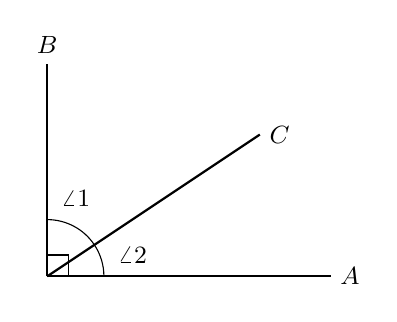
\begin{tikzpicture}[scale=0.9]
  \draw[thick] (0,0) -- (4,0);
  \draw[thick] (0,0) -- (0,3);
  \draw[thick] (0,0) -- (3,2);
  \draw (0.8,0) arc[start angle=0,end angle=34,radius=0.8];
  \node at (1.2,0.3) {\small $\angle 2$};
  \draw (0,0.8) arc[start angle=90,end angle=34,radius=0.8];
  \node at (0.4,1.1) {\small $\angle 1$};
  \node[right] at (4,0) {\small $A$};
  \node[above] at (0,3) {\small $B$};
  \node[right] at (3,2) {\small $C$};
  % Right angle mark
  \draw (0.3,0) -- (0.3,0.3) -- (0,0.3);
\end{tikzpicture}
\end{center}
\end{questionText}
\choiceA{$27°$}
\choiceB{$37°$}
\choiceC{$53°$}
\choiceD{$127°$}
\correctAnswer{B}
\explanation{The two angles together form a right angle ($90°$). $90° - 53° = 37°$.}
\end{practiceQuestion}

\begin{practiceQuestion}{6-7-q15}{mc}
\begin{questionText}
Point $L(-1, -4)$ is reflected over the $y$-axis and then translated up $3$. What are the final coordinates?
\end{questionText}
\choiceA{$(1, -1)$}
\choiceB{$(-1, -1)$}
\choiceC{$(1, -7)$}
\choiceD{$(-1, 1)$}
\correctAnswer{A}
\explanation{Reflect over $y$-axis: $(-1, -4) \to (1, -4)$. Translate up $3$: $(1, -4 + 3) = (1, -1)$.}
\end{practiceQuestion}

\begin{practiceQuestion}{6-8-q04}{mc}
\begin{questionText}
Triangle $PQR \sim$ Triangle $STU$. $PQ = 8$, $ST = 20$, $QR = 6$. Find $TU$.
\end{questionText}
\choiceA{$10$}
\choiceB{$12$}
\choiceC{$15$}
\choiceD{$18$}
\correctAnswer{C}
\explanation{Scale factor: $\frac{20}{8} = 2.5$. $TU = 6 \times 2.5 = 15$.}
\end{practiceQuestion}

\begin{practiceQuestion}{7-4-q17}{mc}
\begin{questionText}
A swimming pool is shaped like a rectangle $25$ m by $10$ m with a semicircle of diameter $10$ m at one end. What is the total area? Use $\pi \approx 3.14$.
\end{questionText}
\choiceA{$250$ m$^2$}
\choiceB{$289.25$ m$^2$}
\choiceC{$328.5$ m$^2$}
\choiceD{$367.75$ m$^2$}
\correctAnswer{B}
\explanation{Rectangle: $25 \times 10 = 250$ m$^2$. Semicircle: $\frac{1}{2} \times 3.14 \times 5^2 = \frac{1}{2} \times 78.5 = 39.25$ m$^2$. Total: $250 + 39.25 = 289.25$ m$^2$.}
\end{practiceQuestion}

\begin{practiceQuestion}{7-5-q26}{gmc}
\begin{questionText}
The net of a rectangular prism is shown below. What is the total surface area?

\begin{center}
\begin{tikzpicture}[scale=0.4]
  % Base cross-shaped net
  \draw[thick,funBlue,fill=funBlue!10] (0,0) rectangle (6,4);
  \node at (3,2) {$6 \times 4$};
  \draw[thick,funBlue,fill=funBlue!10] (6,0) rectangle (9,4);
  \node at (7.5,2) {$3 \times 4$};
  \draw[thick,funBlue,fill=funBlue!10] (9,0) rectangle (15,4);
  \node at (12,2) {$6 \times 4$};
  \draw[thick,funBlue,fill=funBlue!10] (15,0) rectangle (18,4);
  \node at (16.5,2) {$3 \times 4$};
  \draw[thick,funBlue,fill=funBlue!10] (0,4) rectangle (6,7);
  \node at (3,5.5) {$6 \times 3$};
  \draw[thick,funBlue,fill=funBlue!10] (0,-3) rectangle (6,0);
  \node at (3,-1.5) {$6 \times 3$};
\end{tikzpicture}
\end{center}
\end{questionText}
\choiceA{$72$ square units}
\choiceB{$84$ square units}
\choiceC{$108$ square units}
\choiceD{$144$ square units}
\correctAnswer{C}
\explanation{Two $6 \times 4$ faces: $48$. Two $3 \times 4$ faces: $24$. Two $6 \times 3$ faces: $36$. Total: $48 + 24 + 36 = 108$ square units.}
\end{practiceQuestion}

\begin{practiceQuestion}{7-6-q20}{sa}
\begin{questionText}
A cube has a side length of $6$ inches. What is its volume?
\end{questionText}
\correctAnswer{$216$ in$^3$}
\explanation{$V = 6^3 = 216$ in$^3$.}
\end{practiceQuestion}

\begin{practiceQuestion}{7-7-q16}{mc}
\begin{questionText}
A label is wrapped around a can with radius $4$ cm and height $10$ cm. What is the area of the label (the lateral surface only)? Use $\pi \approx 3.14$.
\end{questionText}
\choiceA{$50.24$ cm$^2$}
\choiceB{$125.6$ cm$^2$}
\choiceC{$251.2$ cm$^2$}
\choiceD{$351.68$ cm$^2$}
\correctAnswer{C}
\explanation{Lateral area $= 2\pi rh = 2 \times 3.14 \times 4 \times 10 = 251.2$ cm$^2$.}
\end{practiceQuestion}

\begin{practiceQuestion}{8-1-q30}{gsa}
\begin{questionText}
The table shows the results of a random sample of $80$ people about their preferred pet.

\begin{center}
\begin{tabular}{|l|c|}
\hline
\textbf{Pet} & \textbf{Number} \\
\hline
Dog & $32$ \\
\hline
Cat & $24$ \\
\hline
Fish & $12$ \\
\hline
Bird & $8$ \\
\hline
Other & $4$ \\
\hline
\end{tabular}
\end{center}

What percent of the sample prefers cats? If the population is $5{,}000$, predict how many prefer cats.
\end{questionText}
\correctAnswer{$30\%$; $1{,}500$ people}
\explanation{$\frac{24}{80} = 0.30 = 30\%$. Then $30\%$ of $5{,}000 = 1{,}500$.}
\end{practiceQuestion}

\begin{practiceQuestion}{8-3-q01}{mc}
\begin{questionText}
Class A has a mean test score of $78$ and Class B has a mean test score of $85$. What can you conclude?
\end{questionText}
\choiceA{Every student in Class B scored higher than every student in Class A}
\choiceB{Class B scored higher on average than Class A}
\choiceC{Class A and Class B have the same scores}
\choiceD{Class A has more students than Class B}
\correctAnswer{B}
\explanation{The mean tells us the average performance. Class B scored higher on average, but individual scores may overlap.}
\end{practiceQuestion}

\begin{practiceQuestion}{8-4-q14}{mc}
\begin{questionText}
Data: $42, 45, 47, 50, 53, 55, 58$. Find $Q_1$ and $Q_3$.
\end{questionText}
\choiceA{$Q_1 = 45$, $Q_3 = 55$}
\choiceB{$Q_1 = 42$, $Q_3 = 58$}
\choiceC{$Q_1 = 47$, $Q_3 = 53$}
\choiceD{$Q_1 = 44$, $Q_3 = 56$}
\correctAnswer{A}
\explanation{Median $= 50$. Lower half: $42, 45, 47$, so $Q_1 = 45$. Upper half: $53, 55, 58$, so $Q_3 = 55$.}
\end{practiceQuestion}

\begin{practiceQuestion}{8-5-q03}{mc}
\begin{questionText}
A stem-and-leaf plot has the row: $3 \mid 1\;4\;4\;7\;9$. How many data values are in this row?
\end{questionText}
\choiceA{$3$}
\choiceB{$4$}
\choiceC{$5$}
\choiceD{$25$}
\correctAnswer{C}
\explanation{Count the leaves: $1, 4, 4, 7, 9$ — that's $5$ data values ($31, 34, 34, 37, 39$).}
\end{practiceQuestion}

\begin{practiceQuestion}{9-3-q21}{sa}
\begin{questionText}
A basketball player attempted $80$ free throws and made $56$. What is the experimental probability that she makes her next free throw? Write your answer as a decimal.
\end{questionText}
\correctAnswer{$0.7$}
\explanation{$P = \frac{56}{80} = 0.7$.}
\end{practiceQuestion}

\begin{practiceQuestion}{9-6-q26}{gmc}
\begin{questionText}
The table shows all possible sums when two dice are rolled. What is the probability of rolling a sum of $8$?

\begin{center}
\begin{tabular}{|c|c|c|c|c|c|c|}
\hline
$+$ & \textbf{1} & \textbf{2} & \textbf{3} & \textbf{4} & \textbf{5} & \textbf{6} \\
\hline
\textbf{1} & $2$ & $3$ & $4$ & $5$ & $6$ & $7$ \\
\hline
\textbf{2} & $3$ & $4$ & $5$ & $6$ & $7$ & \cellcolor{funBlue!20}$8$ \\
\hline
\textbf{3} & $4$ & $5$ & $6$ & $7$ & \cellcolor{funBlue!20}$8$ & $9$ \\
\hline
\textbf{4} & $5$ & $6$ & $7$ & \cellcolor{funBlue!20}$8$ & $9$ & $10$ \\
\hline
\textbf{5} & $6$ & $7$ & \cellcolor{funBlue!20}$8$ & $9$ & $10$ & $11$ \\
\hline
\textbf{6} & $7$ & \cellcolor{funBlue!20}$8$ & $9$ & $10$ & $11$ & $12$ \\
\hline
\end{tabular}
\end{center}
\end{questionText}
\choiceA{$\frac{4}{36}$}
\choiceB{$\frac{5}{36}$}
\choiceC{$\frac{6}{36}$}
\choiceD{$\frac{8}{36}$}
\correctAnswer{B}
\explanation{Outcomes with sum $8$: $(2,6), (3,5), (4,4), (5,3), (6,2)$ — that is $5$. $P = \frac{5}{36}$.}
\end{practiceQuestion}

\begin{practiceQuestion}{9-7-q18}{mc}
\begin{questionText}
In a simulation of $100$ free throws, a basketball player makes $78$. If the player's actual success rate is $75\%$, is the simulation result reasonable?
\end{questionText}
\choiceA{No, any difference means the simulation is wrong}
\choiceB{Yes, $78\%$ is close to $75\%$, which is expected variation}
\choiceC{No, because $78$ is not equal to $75$}
\choiceD{Yes, but only if exactly $75$ are made}
\correctAnswer{B}
\explanation{$\frac{78}{100} = 0.78$ vs. theoretical $0.75$. A small difference in $100$ trials is normal and expected.}
\end{practiceQuestion}
